\section{Dissertation overview}
\label{sec:Dissertation overview}
%.5 page
This dissertation comprises six chapters, beginning with this introduction chapter \ref{chap:Introduction}, presenting the research background, aims and ethics, followed by the literature review chapter \ref{chap:Literature review}, which comprehensively reviews previous researches on deep learning models and the related state-of-the-art works.
In chapter \ref{chap:Design}, this dissertation proposes the deep learning model used to recognise and classify actions, based on various designing trade-offs and mobile optimisation methods learned from previous research.
Figure \ref{fig:0-Intro-Overview} shows the project overview, in which these process pipelines and the proposed deep learning model are implemented in chapter \ref{chap:Implementation}.
Further, the experiments are conducted

\begin{figure}[h]
    \centering
    \hspace*{-.5cm}
    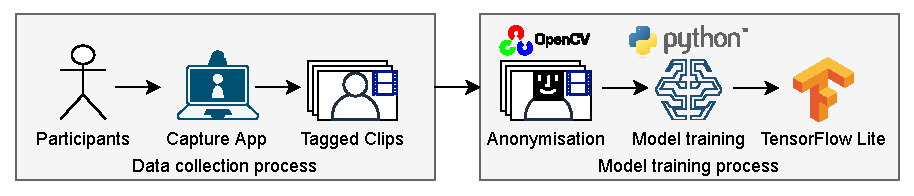
\includegraphics[scale=1.1]{introduction/imgs/0-Intro-Overview.pdf}
    \caption{Project overview}
    \label{fig:0-Intro-Overview}
\end{figure}